\documentclass[tikz,border=1pt]{standalone}
\usepackage{newtxtext,newtxmath}
\usetikzlibrary{positioning,arrows.meta,fit,backgrounds,calc}
% palette (validated): blue #2A78D6, orange #EB6834, aqua #1BAF7A
\definecolor{sblue}{HTML}{2A78D6}\definecolor{sorange}{HTML}{EB6834}\definecolor{saqua}{HTML}{1BAF7A}
\definecolor{ink}{HTML}{0B0B0B}\definecolor{ink2}{HTML}{52514E}\definecolor{muted}{HTML}{8A8984}
\definecolor{surf}{HTML}{F4F3F0}\definecolor{bluebg}{HTML}{EAF2FC}\definecolor{orangebg}{HTML}{FDEEE7}
\colorlet{aquabg}{saqua!12!white}
\newcommand{\GLWE}{\mathrm{GLWE}}\newcommand{\GGSW}{\mathrm{GGSW}}
\newcommand{\tk}{\mathsf{tk}}
\begin{document}
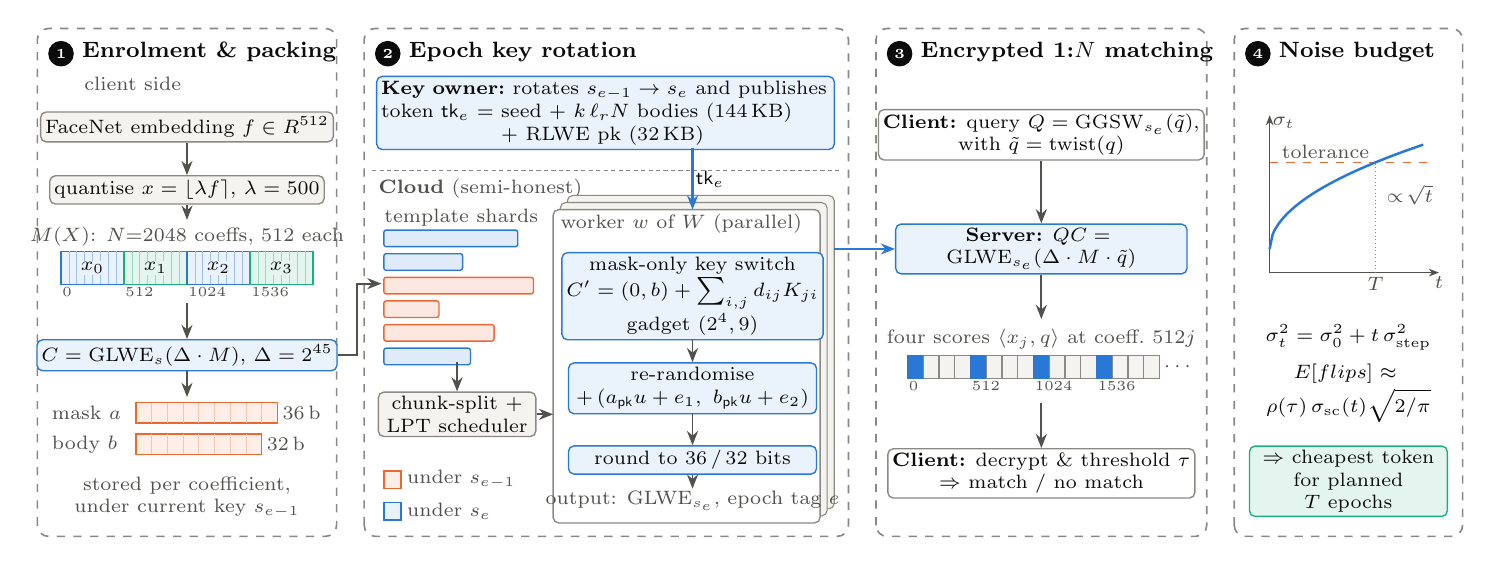
\begin{tikzpicture}[x=1mm,y=1mm,
  font=\scriptsize, text=ink, >={Stealth[length=1.8mm,width=1.4mm]},
  panel/.style={draw=muted, dashed, line width=0.6pt, rounded corners=4pt},
  ptitle/.style={font=\footnotesize\bfseries, anchor=north west, inner sep=0},
  box/.style={draw=muted, line width=0.5pt, rounded corners=2pt, fill=white, align=center, inner sep=1.6pt, text=ink},
  bbox/.style={box, draw=sblue, fill=bluebg},
  obox/.style={box, draw=sorange, fill=orangebg},
  sbox/.style={box, fill=surf},
  lbl/.style={font=\scriptsize, text=ink2, align=center, inner sep=0.8pt},
  tlbl/.style={font=\tiny, text=ink2, align=center, inner sep=0.8pt},
  flow/.style={->, line width=0.7pt, draw=ink2},
  bflow/.style={->, line width=0.9pt, draw=sblue},
  cnum/.style={circle, draw=ink, fill=ink, text=white, font=\tiny\bfseries, inner sep=0.3pt, minimum size=3.1mm},
]
\def\H{66}\def\B{1.5}
% ================= panel frames =================
\def\aL{0}\def\aR{38}
\def\bL{41.5}\def\bR{103}
\def\cL{106.5}\def\cR{148.5}
\def\dL{152}\def\dR{181}
\draw[panel] (\aL,\B) rectangle (\aR,\H);
\draw[panel] (\bL,\B) rectangle (\bR,\H);
\draw[panel] (\cL,\B) rectangle (\cR,\H);
\draw[panel] (\dL,\B) rectangle (\dR,\H);
\node[cnum] at (\aL+3,\H-3.2) {1}; \node[ptitle] at (\aL+5.6,\H-1.6) {Enrolment \& packing};
\node[cnum] at (\bL+3,\H-3.2) {2}; \node[ptitle] at (\bL+5.6,\H-1.6) {Epoch key rotation};
\node[cnum] at (\cL+3,\H-3.2) {3}; \node[ptitle] at (\cL+5.6,\H-1.6) {Encrypted 1:$N$ matching};
\node[cnum] at (\dL+3,\H-3.2) {4}; \node[ptitle] at (\dL+5.6,\H-1.6) {Noise budget};

% ================= panel 1 =================
\def\ac{19}
\node[lbl, anchor=north west] at (\aL+5.6,\H-5.8) {client side};
\node[sbox, minimum width=33mm] (emb) at (\ac,53.5) {FaceNet embedding $f\in\mathbb{R}^{512}$};
\node[sbox, minimum width=33mm] (qnt) at (\ac,45.5) {quantise $x=\lfloor \lambda f\rceil$,\ $\lambda=500$};
\draw[flow] (emb) -- (qnt);
% packed polynomial: 4 blocks of 512 coefficients
\def\gx{3}\def\gw{8}\def\gy{33.5}
\node[lbl, anchor=south] at (\ac,\gy+4.5) {$M(X)$: $N{=}2048$ coeffs, 512 each};
\foreach \j/\fc/\dc in {0/bluebg/sblue,1/aquabg/saqua,2/bluebg/sblue,3/aquabg/saqua}{
  \draw[draw=\dc, fill=\fc, line width=0.5pt] (\gx+\j*\gw,\gy) rectangle ++(\gw,4.2);
  \foreach \k in {1,...,7}{\draw[\dc!45, line width=0.25pt] (\gx+\j*\gw+\k,\gy) -- ++(0,4.2);}
  \node[fill=\fc, inner sep=0.4pt, font=\scriptsize] at (\gx+\j*\gw+\gw/2,\gy+2.1) {$x_{\j}$};
}
\foreach \j/\t in {0/0,1/512,2/1024,3/1536}{\node[tlbl, anchor=north west, inner sep=0.3pt] at (\gx+\j*\gw,\gy-0.2) {\t};}
\draw[flow] (qnt) -- (\ac,\gy+8.2);
\node[bbox, minimum width=33mm] (enc) at (\ac,24.5) {$C=\GLWE_{s}(\Delta\cdot M)$,\ $\Delta=2^{45}$};
\draw[flow] (\ac,\gy-2.4) -- (enc);
% storage bars
\def\bx{12.5}
\node[lbl, anchor=west] at (1.5,17.2) {mask $a$};
\draw[draw=sorange, fill=orangebg, line width=0.5pt] (\bx,15.9) rectangle (\bx+18,18.5);
\foreach \k in {1,...,8}{\draw[sorange!40, line width=0.25pt] (\bx+\k*2,15.9) -- ++(0,2.6);}
\node[lbl, anchor=west] at (\bx+18.3,17.2) {36\,b};
\node[lbl, anchor=west] at (1.5,13.2) {body $b$};
\draw[draw=sorange, fill=orangebg, line width=0.5pt] (\bx,11.9) rectangle (\bx+16,14.5);
\foreach \k in {1,...,7}{\draw[sorange!40, line width=0.25pt] (\bx+\k*2,11.9) -- ++(0,2.6);}
\node[lbl, anchor=west] at (\bx+16.3,13.2) {32\,b};
\draw[flow] (enc) -- (\ac,19.2);
\node[lbl] at (\ac,6.5) {stored per coefficient,\\ under current key $s_{e-1}$};

% ================= panel 2 =================
\node[box, draw=sblue, fill=bluebg, anchor=north west, text width=57mm, align=left] (owner) at (\bL+1.5,\H-6) {%
  \textbf{Key owner:}\ rotates $s_{e-1}\to s_e$ and publishes\\[0.3pt]
  token $\tk_e$ = seed + $k\,\ell_r N$ bodies (144\,KB)\\[0.3pt]
  \phantom{token $\tk_e$ =} + RLWE pk (32\,KB)};
\draw[muted, line width=0.4pt, dash pattern=on 1.5pt off 1.2pt] (\bL+1,48) -- (\bR-1,48);
\node[lbl, anchor=north west] at (\bL+1.5,47.3) {\textbf{Cloud} (semi-honest)};
% shards of unequal size
\def\sx{\bL+2.5}
\foreach \i/\len/\c in {0/17/sblue,1/10/sblue,2/19/sorange,3/7/sorange,4/14/sorange,5/11/sblue}{
  \draw[draw=\c, fill=\c!15!white, line width=0.5pt, rounded corners=0.8pt] (\sx,38.3-\i*3) rectangle ++(\len,2.1);
}
\node[lbl, anchor=north west, inner sep=0] at (\sx,43.2) {template shards};
% scheduler
\node[sbox, minimum width=20mm] (sched) at (\bL+11.8,17) {chunk-split +\\ LPT scheduler};
\draw[flow] (\bL+11.8,23.6) -- (sched.north);
% legend
\draw[draw=sorange, fill=orangebg, line width=0.5pt] (\sx,7.6) rectangle ++(2.2,2.2);
\node[lbl, anchor=west] at (\sx+2.6,8.7) {under $s_{e-1}$};
\draw[draw=sblue, fill=bluebg, line width=0.5pt] (\sx,3.6) rectangle ++(2.2,2.2);
\node[lbl, anchor=west] at (\sx+2.6,4.7) {under $s_e$};
% workers (stacked cards)
\def\wL{\bL+24}\def\wR{\bR-3.6}
\foreach \o in {2,1}{\draw[draw=muted, fill=surf, line width=0.4pt, rounded corners=2pt] (\wL+\o*0.9,3.2+\o*0.9) rectangle (\wR+\o*0.9,43+\o*0.9);}
\draw[draw=muted, fill=white, line width=0.5pt, rounded corners=2pt] (\wL,3.2) rectangle (\wR,43) ;
\node[lbl, anchor=north west] at (\wL+0.6,42.8) {worker $w$ of $W$ (parallel)};
\def\wc{\bL+24+17.7}
\node[bbox, minimum width=31.5mm] (ks) at (\wc,32) {mask-only key switch\\[0.3pt]
  $C'=(0,b)+\sum_{i,j} d_{ij}K_{ji}$\\[0.3pt]gadget $(2^4,9)$};
\node[bbox, minimum width=31.5mm] (rr) at (\wc,20.3) {re-randomise\\[0.3pt]$+\,(a_{\mathsf{pk}}u+e_1,\ b_{\mathsf{pk}}u+e_2)$};
\node[bbox, minimum width=31.5mm] (rd) at (\wc,11.2) {round to 36\,/\,32 bits};
\node[lbl] (tag) at (\wc,6) {output: $\GLWE_{s_e}$, epoch tag $e$};
\draw[flow] (ks) -- (rr); \draw[flow] (rr) -- (rd); \draw[flow] (rd) -- (tag);
\draw[flow] (sched.east) -- (\wL,17);
% token arrow
\draw[bflow] (\wc,\H-6-9.2) -- node[lbl, right, pos=0.5, text=ink]{$\tk_e$} (\wc,43);
% ================= panel 1 -> 2 =================
\draw[flow] (enc.east) -- ++(2.5,0) |- (\sx-0.3,33.6);
% ================= panel 3 =================
\def\pc{127.5}
\node[box, minimum width=37mm] (qry) at (\pc,52.5) {\textbf{Client:} query $Q=\GGSW_{s_e}(\tilde q)$,\\ with $\tilde q=\mathrm{twist}(q)$};
\node[bbox, minimum width=37mm] (srv) at (\pc,38) {\textbf{Server:} $Q\boxdot C={}$\\ $\GLWE_{s_e}(\Delta\cdot M\cdot\tilde q)$};
\draw[flow] (qry) -- (srv);
% coefficient grid: 16 cells, 0/512/1024/1536 highlighted
\def\cx{110.5}\def\cw{2}\def\cy{21.5}
\foreach \k in {0,...,15}{
  \pgfmathtruncatemacro{\hl}{mod(\k,4)==0 ? 1 : 0}
  \ifnum\hl=1 \draw[draw=sblue, fill=sblue, line width=0.4pt] (\cx+\k*\cw,\cy) rectangle ++(\cw,3);
  \else \draw[draw=muted, fill=surf, line width=0.4pt] (\cx+\k*\cw,\cy) rectangle ++(\cw,3); \fi
}
\node[lbl, anchor=west] at (\cx+16*\cw+0.2,\cy+1.5) {$\cdots$};
\foreach \k/\t in {0/0,4/512,8/1024,12/1536}{\node[tlbl, anchor=north west, inner sep=0.3pt] at (\cx+\k*\cw,\cy-0.2) {\t};}
\node[lbl, anchor=south] at (\pc,\cy+3.4) {four scores $\langle x_j,q\rangle$ at coeff.\ $512j$};
\draw[flow] (srv) -- (\pc,\cy+7.6);
\node[box, minimum width=37mm] (dec) at (\pc,9.5) {\textbf{Client:} decrypt \& threshold $\tau$\\ $\Rightarrow$ match / no match};
\draw[flow] (\pc,\cy-3) -- (dec);
% panel 2 -> 3
\draw[bflow] (\wR+1.8,38) -- (srv.west);
% ================= panel 4 =================
\def\PFx{156.5}\def\PFy{35}
\draw[->, line width=0.5pt, ink2, >={Stealth[length=1.3mm]}] (\PFx,\PFy) -- (\PFx+21.5,\PFy) node[lbl, anchor=north, inner sep=0.8pt, yshift=-0.2mm]{$t$};
\draw[->, line width=0.5pt, ink2, >={Stealth[length=1.3mm]}] (\PFx,\PFy) -- (\PFx,\PFy+20) node[lbl, anchor=west, inner sep=0.8pt, yshift=-1mm]{$\sigma_t$};
\draw[sorange, dashed, line width=0.6pt] (\PFx,\PFy+14) -- (\PFx+20.5,\PFy+14);
\node[lbl, anchor=south west] at (\PFx+1.2,\PFy+14.2) {tolerance};
\draw[sblue, line width=0.9pt, domain=0:19.5, samples=50, smooth] plot (\PFx+\x, {\PFy+3+3*sqrt(\x)});
\pgfmathsetmacro{\PFt}{(11/3)^2}
\draw[muted, line width=0.3pt, densely dotted] (\PFx+\PFt,\PFy) -- (\PFx+\PFt,\PFy+14);
\node[lbl, anchor=north] at (\PFx+\PFt,\PFy-0.2) {$T$};
\node[lbl, anchor=north west] at (\PFx+14.5,\PFy+11.5) {$\propto\!\sqrt{t}$};
\node[anchor=north, align=center, font=\scriptsize, inner sep=0] at (166.5,28.5) {$\sigma_t^2=\sigma_0^2+t\,\sigma_{\mathrm{step}}^2$\\[4pt]
  $\mathbb{E}[\text{flips}]\approx{}$\\[1pt]$\rho(\tau)\,\sigma_{\mathrm{sc}}(t)\sqrt{2/\pi}$};
\node[box, draw=saqua, fill=aquabg, text width=24mm] at (166.5,8.5) {$\Rightarrow$ cheapest token\\ for planned $T$ epochs};
\end{tikzpicture}
\end{document}
